\chapter{Topologie dronu}

Práce se zaobírá v první řadě simulací bezpilotních letadel ve virtuálním prostředí, ale z důvodu možné budoucí realizace projektu je nutné pracovat s konkrétními hardwarovými a softwarovými řešeními.

Topologii řídícího systému dronu jsme rozdělili na dvě části. Palubní počítač řídí bezplotnou misi a řídící jednotka ovládá kritické procesy v dronu. Na trhu existuje nepřeberné množství různých komponent pro autonomní mise. Na základě existujících projektů, například \textit{Multi Robot Systems Group} z ČVUT \cite{MRS} jsme zvolili modul Pixhawk jako řídící jednotku. Jako palubní počítač, který ovládá samotnou autonomní misi jsme zvolili jednodeskový počítač Raspberry PI.

S touto kombinací jsme schopni řídit velké množství různých autonomních letadel a vozidel jako jsou:

\begin{itemize}
    \item dron v různých konfiguracích
    \item delta \acs{VTOL} (\acl{VTOL})
    \item letadlo v různých konfiguracích
    \item vrtulník
    \item rover
    \item ponorka
\end{itemize}

\section{Řídící jednotka Pixhawk}

Pixhawk je otevřený hardwarový projekt, jehož cílem je poskytnout standard pro snadno dostupné a vysoce kvalitní návrhy hardwaru autopilota pro akademické, hobby a vývojářské komunity. \cite{PIX1}

Řídící jednotka Pixhawk řídí kritické procesy v dronu jako \textit{fail safe} funkce, ovládání pohonů, stabilizace a čtení kritických snímačů (GPS, barometr) pro řízení dronu.

Existuje několik 

\begin{itemize}
    \item Pixhawk (výroba byla ukončena)
    \item Pixhawk 2 (výroba byla ukončena)
    \item Pixhawk 3 Pro
    \item Pixhawk 4
    \item Pixhawk 4 Mini
    \item Pixhawk 5X
    \item Pixracer
    \item Auterion Skynode (průmyslové řešení)
\end{itemize}

\begin{figure}[!ht]
    \begin{center}
        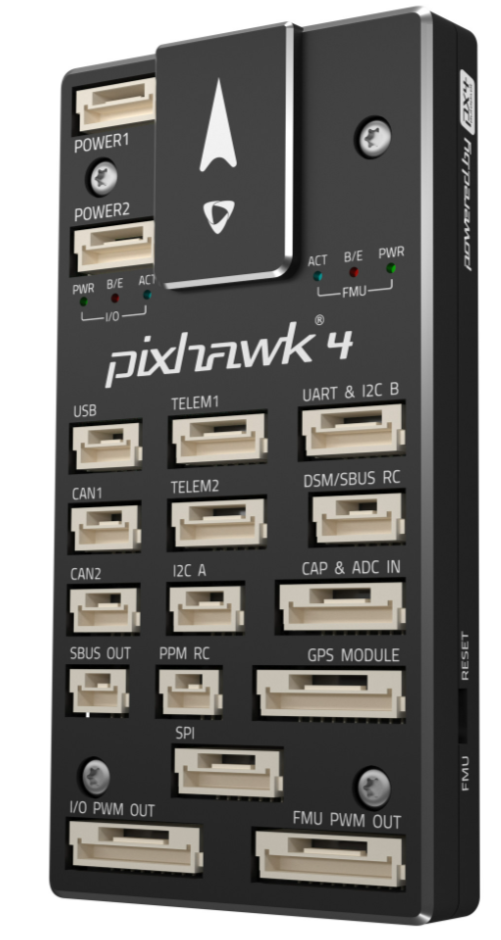
\includegraphics[scale=0.47]{obrazky/PIX}
    \end{center}
    \caption[Řídící jednotka Pixhawk 4]{Řídící jednotka Pixhawk 4 \cite{PIX2}.}
    \label{fig:PIX}
\end{figure}

\section{Palubní počítač}

Jako palubní počítač se pro experimentální letecké mise využívá jednodeskový počítač Raspberry PI. Na trhu existuje množství různých variant tohoto široce rozšířeného počítače v rozmezí od levného, malého a úsporného  \textit{Raspberry PI Pico} až po vysoce výkonný počítač \textit{Raspberry PI 4}.

Důležitými výhodami pro aplikace v robotických misích jsou integrace na jeden plošní spoj, nízká proudová spotřeba a možnost spuštění linuxových distribucí. Nejběžnější podporované distribuce jsou Raspberry PI OS, Raspbian, Ubuntu desktop a server.

Hlavní důvod pro použití Raspberry PI jako palubního počítače je možnost spolehlivé komunikace s PX4 firmware přes ROS 2 \textit{topic}. Komunikací mezi uvedenými platformami se budeme zabývat v následujících kapitolách.